%%
%% This is file `template-8s.tex',
%% generated with the docstrip utility.
%%
%% The original source files were:
%%
%% template.raw  (with options: `8s')
%% 
%% Template for the LaTeX class aipproc.
%% 
%% (C) 1998,2000,2001 American Institute of Physics and Frank Mittelbach
%% All rights reserved
%% 
%%
%% $Id: template.raw,v 1.12 2005/07/06 19:22:14 frank Exp $
%%

%%%%%%%%%%%%%%%%%%%%%%%%%%%%%%%%%%%%%%%%%%%%
%% Please remove the next line of code if you
%% are satisfied that your installation is
%% complete and working.
%%
%% It is only there to help you in detecting
%% potential problems.
%%%%%%%%%%%%%%%%%%%%%%%%%%%%%%%%%%%%%%%%%%%%

%\input{aipcheck}
%%%%%%%%%%%%%%%%%%%%%%%%%%%%%%%%%%%%%%%%%%%%
%% SELECT THE LAYOUT
%%
%% The class supports further options.
%% See aipguide.pdf for details.
%%
%%%%%%%%%%%%%%%%%%%%%%%%%%%%%%%%%%%%%%%%%%%%

\documentclass[
    ,final            % use final for the camera ready runs
%%  ,draft            % use draft while you are working on the paper
%%  ,numberedheadings % uncomment this option for numbered sections
%%  ,                 % add further options here if necessary
  ]
%  {aipproc}
  
\usepackage{float}
\usepackage{amsmath}
\floatstyle{ruled}
\newfloat{algorithm}{htbp}{loa}
\floatname{algorithm}{Pseudo Code}
\layoutstyle{8x11single}%double}


%%%%%%%%%%%%%%%%%%%%%%%%%%%%%%%%%%%%%%%%%%%%
%% FRONTMATTER
%%%%%%%%%%%%%%%%%%%%%%%%%%%%%%%%%%%%%%%%%%%%

\begin{document}

\title{Design and Development of an Optimised Hardware Encryption module of
gigabit throughput base on Composite Glois Field Arithmetic with Feedback Modes}

\classification{}%{<Replace this text with PACS numbers; choose from this list:
               %\texttt{http://www.aip..org/pacs/index.html}>}
\keywords      {Cryptography, AES, Galois Field, Composite Galois Field, Hardware Implementation (FPGA), Pipeline}

\author{Abhishek Bajpai}{
  address={abbajpai@barc.gov.in}
}

\author{Bhagwan Bathe}{
  address={bathebn@barc.gov.in}
}

\author{S K Parulkar}{
  address={skparul@barc.gov.in}
}

\author{A G Apte}{
  address={apteag@barc.gov.in}
  ,altaddress={Computer Division, BARC, Mumbai} % additional visiting address
}


\begin{abstract}

Performance evaluation of the Advanced Encryption Standard candidates results to intensive study of both hardware and software implementations. However, different implementation designs have been proposed through number of papers though, it seems that efficiency could still be greatly improved by applying good design rules adapted for devices and algorithms. This paper addresses composite field approach for efficient FPGA implementations of the Advanced Encryption Standard algorithm. As different applications of the AES algorithm may require different speed/area trade-offs. In this paper, we have discussed design methodology and algorithmic optimization to improve previously reported results. We also define an optimal pipeline that takes the place and route constraints into account. Resulting circuits significantly improve previously reported results throughput is up to three gigabits/sec and area requirements can be limited to 3k CLB with a ratio throughput/area improved by at least 50\% of the best-known designs in the Xilinx Virtex technology. We also have done a case study for general requirement for high throughput systems and have suggested a multichannel approach for implementing feedback modes without loosing overall throughput. 
\end{abstract}

\maketitle



%%%%%%%%%%%%%%%%%%%%%%%%%%%%%%%%%%%%%%%%%%%%%%%%
%% SECTION
%%%%%%%%%%%%%%%%%%%%%%%%%%%%%%%%%%%%%%%%%%%%%%%%
\section{Introduction}
There is a constant security threat to the information we communicate on public media. Most of the communication is done without or with moderate security. It is required to shift to the secured environment in which the information is conveyed in encrypted form. But this shift is not possible with today's available 8/32 bit processors as encryption algorithm is computational intensive. It is observed \cite{Bernsteinnewaes} that on average a processor architecture takes 22 cycles/byte for AES  encryption resulting throughput of  36.3 Mbps for 100 Mhz clock.

On the other hand hardware approach based on FPGA is bit promising. As algorithm runs parallel in the core and there is a lot of scope for pipe-lining. Modular Hardware based on this approach can give us good solution for our security problems in communication devices. Implementation of an Encryption algorithm on FPGA is not a new concept. But there is a scope in its optimum implementation in hardware. Encryption hardware also gives us functional abstraction for a communicating device as device doesn't have to bother about the security or encryption. And you can always change the algorithm by just reprogramming it.

In this project different approaches for implementing AES encryption have been studied and it has been observed that the most compact design implementations are based on Composite field inversion. Different optimization approaches are also been studied and developed for generating most compact core. For example Sbox and Inverse Sbox are implemented as a single module which share a common core of field inversion. Similarly Mix column and Inverse mix column are also implemented in a single module with deep byte level resource sharing. A new design of Memory mapped State array is discussed which works as an accumulator and can handle 32 bit row as well as 32 bit column transformations. For high throughput these cores can be implemented in parallel topology. Thus giving Giga bit throughput. 128 bit Design is also developed and throughput analysis is done for both designs.
%%%%%%%%%%%%%%%%%%%%%%%%%%%%%%%%%%%%%%%%%%%%%%%%
%% SECTION
%%%%%%%%%%%%%%%%%%%%%%%%%%%%%%%%%%%%%%%%%%%%%%%%
\section{AES Algorithm}
The AES algorithm, also called the Rijndael algorithm, is a symmetric block cipher, where the data is encrypted/decrypted in blocks of 128 bits. Each data block is modified by several rounds of processing, where each round involves four steps. Three different key sizes are allowed: 128 bits, 192 bits, or 256 bits, and corresponding several rounds for each is 10 rounds, 12 rounds, or 14 rounds, respectively. From the original key, a different "round key" is computed for each of these rounds. For simplicity, the discussion below will use a key length of 128 bits and hence 10 rounds.

    There are several different modes in which AES can be used. Some of these, such as Cipher Block Chaining (CBC), use the result of encrypting one block for encrypting the next. These feedback modes effectively preclude pipelining (simultaneous processing of several blocks in the "pipeline"). Other modes, such as the "Electronic Code Book" mode or "Counter" modes, do not require feedback, and may be pipelined for greater throughput.

    The four steps in each round of encryption, in order, are called SubBytes (byte substitution), ShiftRows, MixColumns, and AddRoundKey. Before the first round, the input block is processed by AddRoundKey. Also, the last round skips the MixColumns step. Otherwise, all rounds are the same, except each uses a different round key, and the output of one round becomes the input for the next. For decryption, the mathematical inverse of each step is used, in reverse order; certain manipulations allow this to appear like the same steps as encryption with certain constants changed. Each round key calculation also requires the SubBytes operation. (More complete descriptions of AES are available from several sources, e.g., \cite {Processing_announcingthe})

    Of these four steps, three of them (ShiftRows, MixColumns, and AddRoundKey) are linear, in the sense that the output 128-bit block for such steps are just the linear combination (bitwise, modulo 2) of the outputs for each separate input bit. These three steps are all easy to implement by direct calculation in software or hardware.

    The single nonlinear step is the SubBytes step, where each byte of the input is replaced by the result of applying the "S-box" function to that byte. This nonlinear function involves finding the inverse of the 8-bit number, considered as an element of the Galois field $GF(2^8)$. The Galois inverse is not a simple calculation, and so many current implementations use a table of the S-box function output. This table look-up method is fast and easy to implement.
    
\begin{figure}
  \centering
    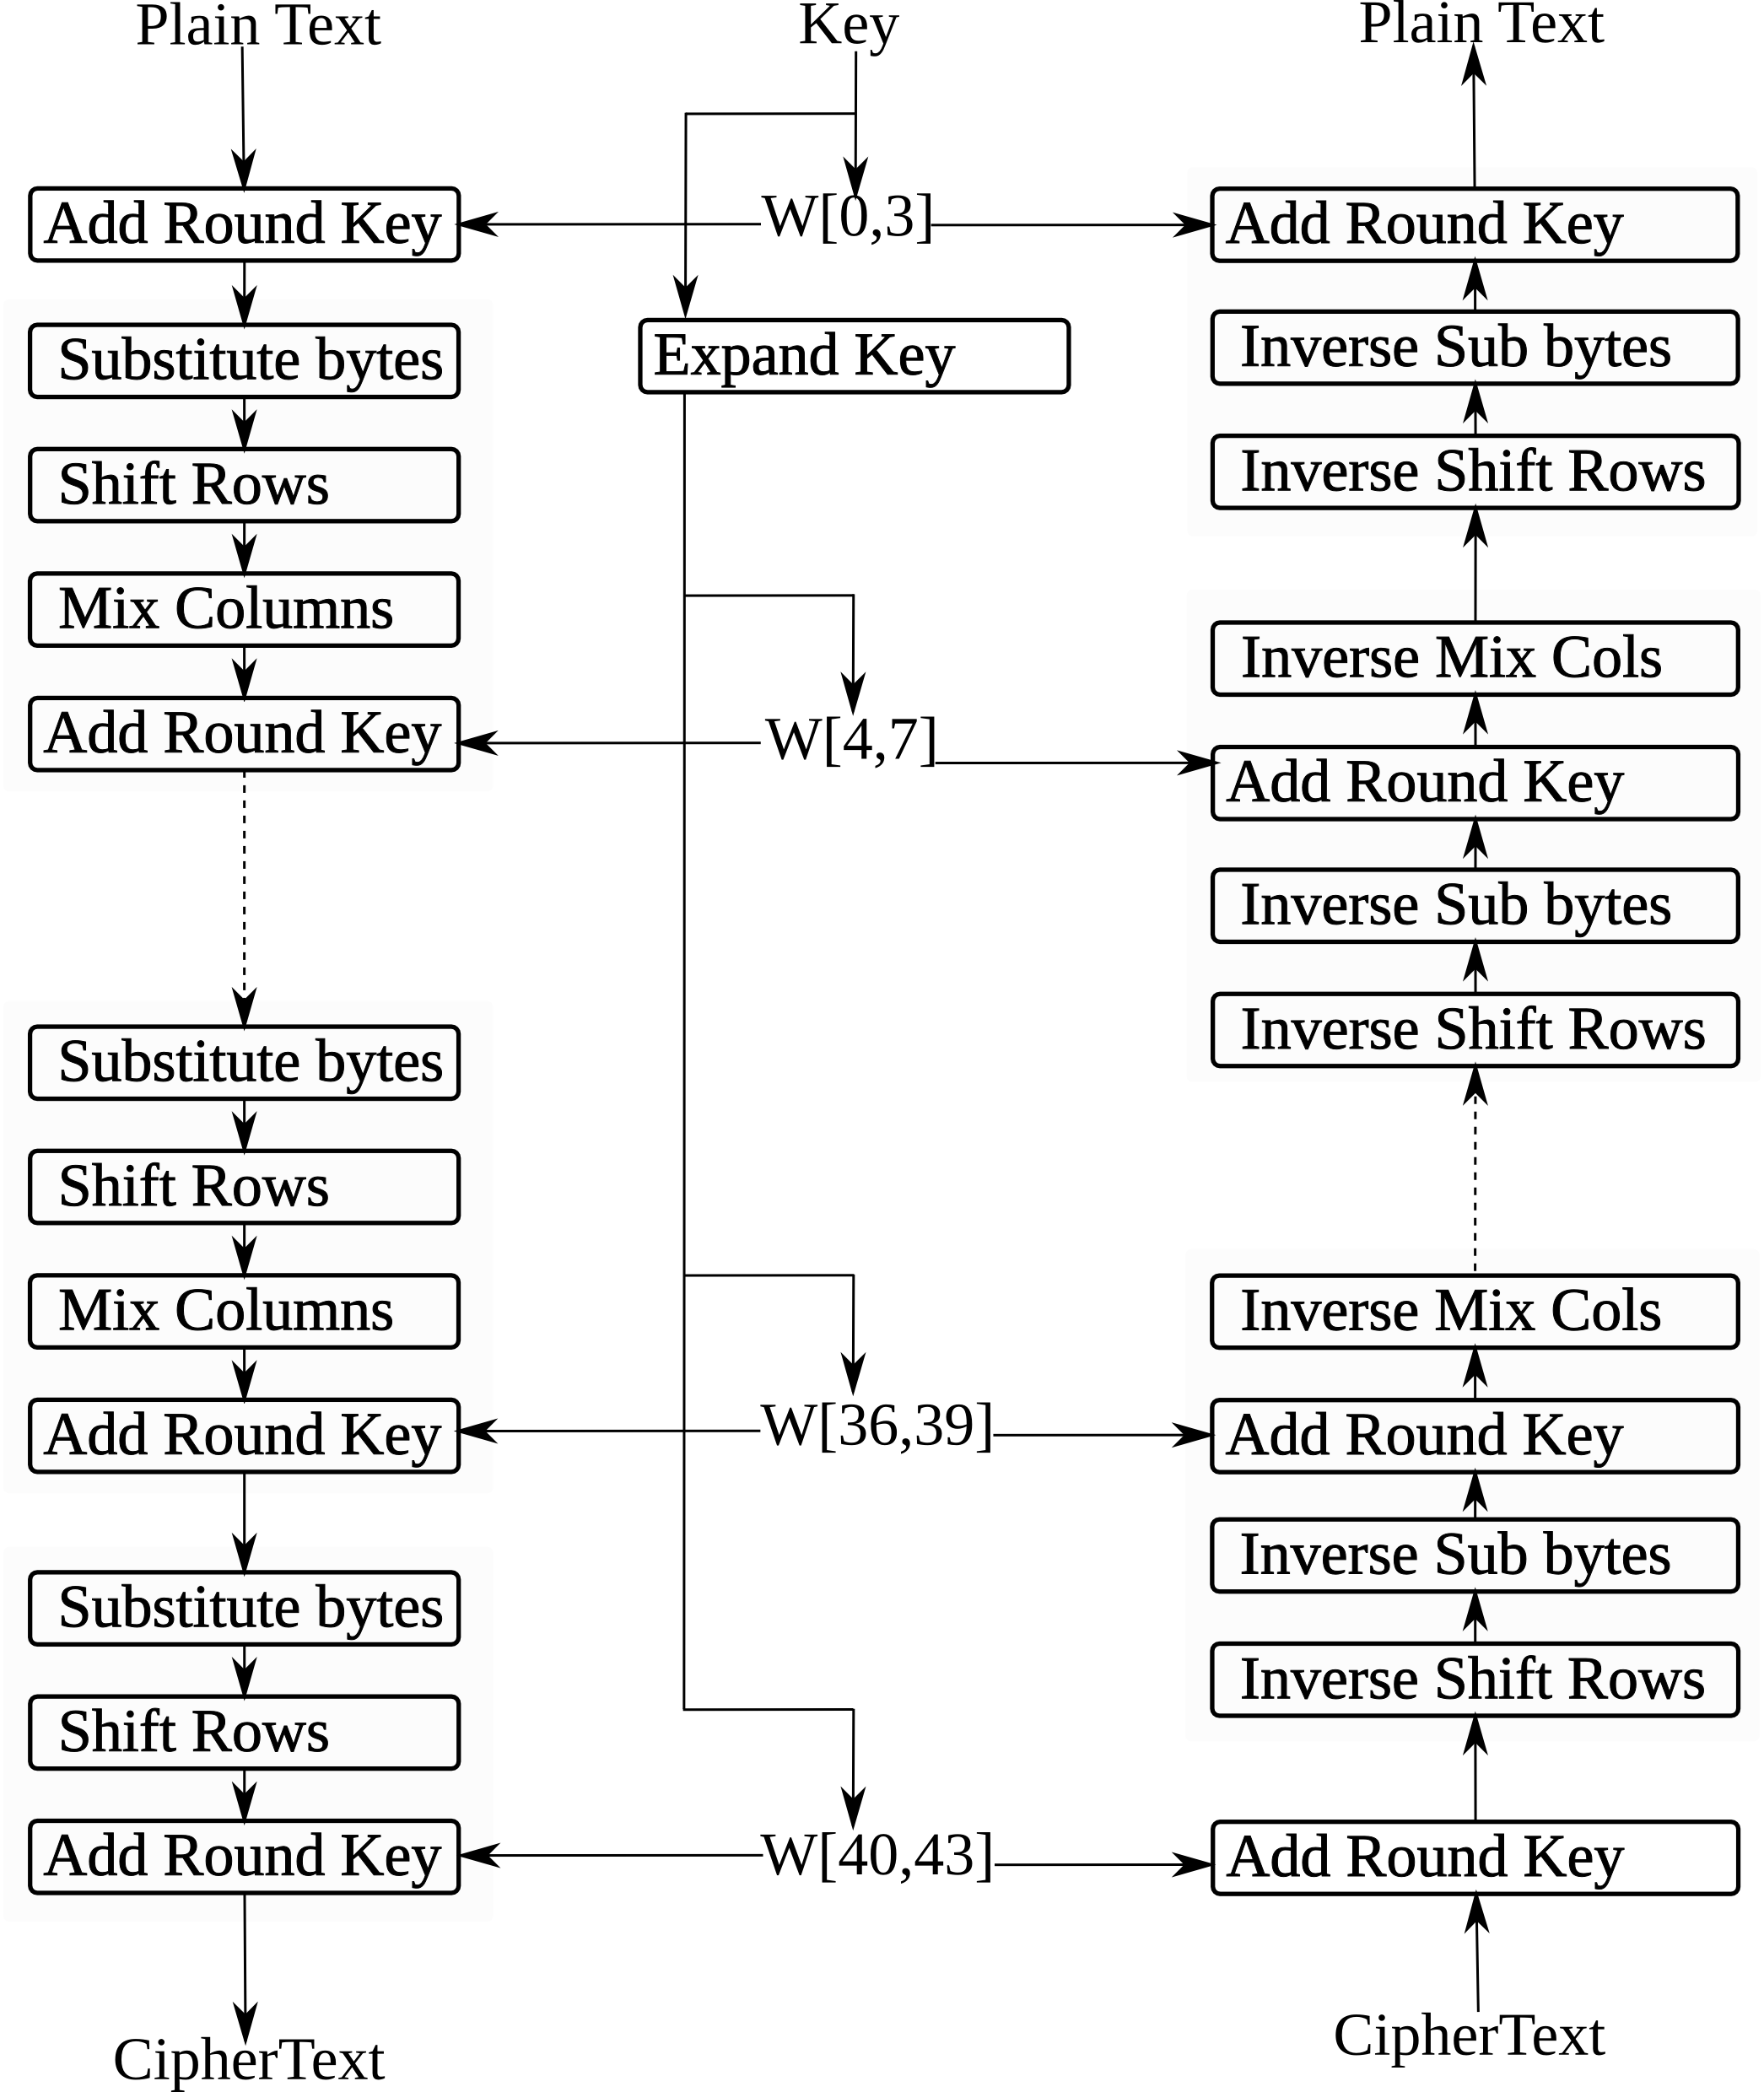
\includegraphics[width=0.50 \textwidth]{mtech/gifs/AES_structure.png}
  \caption{AES Algorithm Flow Diagram\cite{Processing_announcingthe}}
  \label{AES_structure}
\end{figure}
    But for hardware implementations of AES, there is one drawback of the table look-up approach to the S-box function: each copy of the table requires 256 bytes of storage, along with the circuitry to address the table and fetch the results. Each of the 16 bytes in a block can go through the S-box function independently, and so could be processed in parallel for the byte substitution step. This effectively requires 16 copies of the S-box table for one round. To fully pipeline the encryption would entail "unrolling" the loop of 10 rounds into 10 sequential copies of the round calculation. This would require 160 copies of the S-box table (200 if round keys are computed "on the fly"), a significant allocation of hardware resources.


\section{Byte Substitution}\cite{BerkSunar}
The Byte Substitution transformation operates independently on each byte of the state. The operation comprises of 2 sub-steps:  
\begin{enumerate}
\item Inversion: Multiplicative inverse of each byte is taken in $GF(2^8)$, and \{00\} is mapped to itself.
\item Affine Transformation: This sub-step is performed in GF(2).
\end{enumerate}

To implement the Byte Substitution transformation, many techniques have been reported. Those are, for instances; 

\begin{enumerate}
\item The table lookup technique where step 2 is usually combined into a single table known as S-box. Not feasible as discussed.
\item Synthesis and optimized logic function of S-box using CAD tools, and 
\item Compute inversion of element in $GF(2^8)$ and optimize the logic functions. The efficiency of the third technique is much depended on the mathematical theory of field element inversion. This approach is highly considered when the table lookup is not applicable or when the compact design is a case. It also provides desirable features for the highly paralleled computation.
\end{enumerate}

In this project option (3) is chosen since the field inversion hardware can be easily shared by both the encryption process and decryption process. The Byte Substitution (and similarly, the inverse Byte Substitution) transform of a byte is defined mathematically as:

\begin{equation}
D(x) = \delta  A^{-1} (x)_{mod (x^8+1)} \oplus C(x)
\end{equation}


where $C(x)~=~x^6~+~x^5~+~x~+~1~=~\{63\}$ and $\delta~=~\{1F\}~=~x^4~+~x^3~+~x^2~+~x~+~1$. For the inverse Byte Substitution computation, $\delta~=~\{4A\}~=~x^6~+~x^3~+~x$ and $C(x)~=~x^2~+~1~=~\{05\}$ are used respectively. The constant C(x) has been added in order that the Sbox has no fixed point (a map to a) and no opposite fixed point ( a map to \={a} ). Besides the field inversion, such a transformation is fairly simple as the circuit can be built up form an array of XOR gates.



%%%%%%%%%%%%%%%%%%%%%%%%%%%%%%%%%%%%%%%%%%%%%%%%
%% SUBSECTION
%%%%%%%%%%%%%%%%%%%%%%%%%%%%%%%%%%%%%%%%%%%%%%%%
\subsection{$GF(2^8)$ to $GF((2^4)^2)$ transformation\cite{springerRudra}\cite{1149067}}
   AES has adopted $m(x) = x^8 +x^4 +x^3 +x+1$ as its field polynomial. Although such a polynomial is an irreducible but it is not a primitive one. Fortunately, with the field isomorphism property, we can map elements in $GF(2^8)$ as shown in [4] to the composite field $GF((2^4)^2)$ based on the polynomial $w(x)=x^2+x+ \beta ^{14}$ , where $\beta ^{14}=\{09\}$ denotes the element in $GF(2^4)$ of which $I(x) = x^4 + x + 1$ is the primitive irreducible polynomial. Let D be an element in $GF(2^8)$ and A be an element in $GF((2^4)^2)$ , then $A = [T] D$ and $D = [T]^{\_ 1} A$
   
where
\begin{equation}
T = \left[ \begin{array}{cccccccc}
1 & 0 & 1 & 1 & 1 & 0 & 1 & 1 \\
0 & 1 & 0 & 1 & 0 & 0 & 0 & 0 \\
0 & 1 & 0 & 0 & 1 & 0 & 1 & 0 \\
0 & 1 & 1 & 0 & 0 & 0 & 1 & 1 \\
0 & 0 & 0 & 0 & 1 & 1 & 1 & 0 \\
0 & 1 & 0 & 0 & 1 & 0 & 1 & 1 \\
0 & 0 & 1 & 1 & 0 & 1 & 0 & 1 \\
0 & 0 & 0 & 0 & 0 & 1 & 0 & 1 \\
 \end{array} \right] 
\end{equation}
and
\begin{equation}
T^{-1} = \left[ \begin{array}{cccccccc}
1 & 0 & 0 & 0 & 1 & 0 & 1 & 0 \\
0 & 0 & 0 & 0 & 1 & 1 & 0 & 1 \\
0 & 1 & 0 & 0 & 1 & 1 & 1 & 0 \\
0 & 1 & 0 & 0 & 1 & 1 & 0 & 1 \\
0 & 1 & 0 & 1 & 1 & 0 & 1 & 0 \\
0 & 0 & 1 & 0 & 0 & 1 & 0 & 1 \\
0 & 1 & 1 & 1 & 0 & 1 & 1 & 1 \\
0 & 0 & 1 & 0 & 0 & 1 & 0 & 0 \\
 \end{array} \right]
\end{equation}
Here $[T]$ and $[T]^{\_ 1}$ are the field transformation matrices. The
upper-left element in the above matrices denotes the least significant bit. In
the composite field, let a byte-format data be expressed as
\begin{equation}
A=\{pq\}=px+q
\end{equation}

%%%%%%%%%%%%%%%%%%%%%%%%%%%%%%%%%%%%%%%%%%%%%%%%
%% SUBSECTION
%%%%%%%%%%%%%%%%%%%%%%%%%%%%%%%%%%%%%%%%%%%%%%%%
\subsection {$G(2^4)^2$ Inversion}
Insted of eculiden There is an another way to calculate $G(2^4)^2$ inverse. Let suppose
\begin{equation}
B =  A^{-1}~~ where~~ A,B~~  in ~~GF(2^4)^2
\end{equation}
so
\begin{equation}
A = a_1 X + a_0
\end{equation}
and
\begin{equation}
B = b_1 X + b_0
\end{equation}
as
\begin{equation}
B = A^{-1}
\end{equation}
\begin{eqnarray}
&&\Rightarrow ~~AB = 1 \nonumber\\
&&\Rightarrow ~~(b_1 X + b_0)(a_1 X + a_0) = 1 \nonumber\\
&&\Rightarrow ~~b_1 a_1 X^2 + (b_1 a_0+b_0 a_1)X + b_0 a_0 = 1
\end{eqnarray}
as
\begin{equation}
X^2 + X + 9 = 0 ~~is~ the~ irreducible~ polynomial \nonumber
\end{equation}
\begin{eqnarray}
&&\Rightarrow ~[b_1 a_1 X^2 + (b_1 a_0+b_0 a_1)X + b_0 a_0] mod_{X^2 + X + \beta^{14} = 1} \nonumber\\
&&\Rightarrow ~[b_1 a_1 X^2 + (b_1 a_0+b_0 a_1)X + b_0 a_0] mod_{X^2 + X  \beta^{14} = 1} \nonumber\\
&&\Rightarrow ~(b_1 a_0+b_0 a_1 + b_1 a_1)X + (b_0 a_0 + b_1 a_1 \beta^{14} )= 1 \nonumber\\
&&\Rightarrow ~(b_1 a_0+b_0 a_1 + b_1 a_1)= 0  \nonumber\\
&&\Rightarrow ~(b_0 a_0 + b_1 a_1 \beta^{14} )= 1  \nonumber\\
&&\Rightarrow ~b_1 = a_1 (a_0^2 + a_1 a_0 +a_1^2 \beta^{14} )^{-1}  \\
&&\Rightarrow ~b_0 = (a_1 + a_0) (a_0^2 + a_1 a_0 +a_1^2 \beta^{14} )^{-1}
\end{eqnarray}
Circuit based on this approach is very promising and will reduce the code by orders.This Inversion only required  two $GF(2^4)$ square three $GF(2^4)$ multiplication and one $GF(2^4)$ inversion. That can be implemented with very few number of gates.

\paragraph{$GF(2^4)$ inverse}
$GF(2^4)$ inverse can be easily implemented as an lookup table.

\begin{table}
	\begin{tabular}{l|r|r|r|r|r|r|r|r|r|r|r|r|r|r|r|r|} 
\hline
  \tablehead{1}{l}{b}{X} 
  & 0x0 & 0x1 & 0x2 & 0x3 & 0x4 & 0x5 & 0x6 & 0x7 & 0x8 & 0x9 & 0xa & 0xb & 0xc & 0xd & 0xe & 0xf\\  
\hline
  \tablehead{1}{r}{b}{$x^{-1}$in GF(4)} 
  & 0x0 & 0x1 & 0x9 & 0xe & 0xd & 0xb & 0x7 & 0x6 & 0xf & 0x2 & 0xc & 0x5 & 0xa & 0x4 & 0x3 & 0x8 \\
\hline
\end{tabular}
\caption{Look up table for G(4) inverse}
\label{tab:lookuptableg4}
\end{table}

\paragraph{$GF(2^4)$ multiplication }
${A_1}^2\beta^{14}$ can also be implemented as an combination logic with the help of only two xor.
\begin{figure}
\centering
\includegraphics[width=0.50 \textwidth]{G4Mul.png}
\caption{Gate Level Implementation of $GF(2^4)$ multiplication}
\label{gf4sqrmul9}
\end{figure}

\paragraph{$GF(2^4)$ square}
$GF(2^4)$ square can be implemented as an combination logic with the help of only two xor.
\begin{figure}
\centering
\includegraphics[width=0.25 \textwidth]{G4Sqa.png}
\caption{Gate Level Implementation of $GF(2^4)$ square}
\label{gf4sqr}
\end{figure}
\paragraph{$GF(2^4)$ square X $\beta^{14}$}
${A_1}^2\beta^{14}$ can also be implemented as an combination logic with the help of only two xor.
\begin{figure}
\centering
\includegraphics[width=0.25 \textwidth]{G4SqaB14.png}
\caption{Gate Level Implementation of $(GF(2^4)^2) \beta^{14}$}
\label{G4SqaB14}
\end{figure}

\subsection{Pipe-lining}
Galois field inversion gives us a very compact design. But design have greater degree of Logic Levels. This design has delay of 13.9 nano seconds. By introducing Pipe-lining Delay is reduced to as low as 3.61 nano Seconds. Refer (table:\ref{tab:b}). At the cost of some small increased gate size and complexities.

\subsection{Affine/Inverse Affine Transformation}
In matrix form, the affine transformation element of the S-box can be expressed as:
\begin{equation}
b(x)=\{1F\}d(x)_{mod (x^8+1)} \oplus c(x)
\end{equation}
where
\begin{equation}
c(x)=\{63\}=x^6+x^5+x+1 \nonumber
\end{equation}
\begin{equation}
\left[ \begin{array}{c}
bo\\b1\\b2\\b3\\b4\\b5\\b6\\b7 \end{array} \right] =
\left[ \begin{array}{cccccccc}
1 & 0 & 0 & 0 & 1 & 1 & 1 & 1\\
1 & 1 & 0 & 0 & 0 & 1 & 1 & 1\\
1 & 1 & 1 & 0 & 0 & 0 & 1 & 1\\
1 & 1 & 1 & 1 & 0 & 0 & 0 & 1\\
1 & 1 & 1 & 1 & 1 & 0 & 0 & 0\\
0 & 1 & 1 & 1 & 1 & 1 & 0 & 0\\
0 & 0 & 1 & 1 & 1 & 1 & 1 & 0\\
0 & 0 & 0 & 1 & 1 & 1 & 1 & 1
 \end{array} \right] \left[ \begin{array}{c}
d_0\\d_1\\d_2\\d_3\\d_4\\d_5\\d_6\\d_7 \end{array} \right]\oplus
 \left[ \begin{array}{c}
1\\1\\0\\0\\0\\1\\1\\0 \end{array} \right]
\end{equation}

the inverse affine transformation element of the S-box can be expressed as:
\begin{equation}
b(x)=\{4A\}d(x)_{mod (x^8+1)}\oplus c(x)
\end{equation} \\ \\
where
\begin{equation}
c(x)=\{05\}=x^2+1 \nonumber
\end{equation}
\begin{equation}
\left[ \begin{array}{c}
bo\\b1\\b2\\b3\\b4\\b5\\b6\\b7 \end{array} \right] =
\left[ \begin{array}{cccccccc}
0 & 0 & 1 & 0 & 0 & 1 & 0 & 1\\
1 & 0 & 0 & 1 & 0 & 0 & 1 & 0\\
0 & 1 & 0 & 0 & 1 & 0 & 0 & 1\\
1 & 0 & 1 & 0 & 0 & 1 & 0 & 0\\
0 & 1 & 0 & 1 & 0 & 0 & 1 & 0\\
0 & 0 & 1 & 0 & 1 & 0 & 0 & 1\\
1 & 0 & 0 & 1 & 0 & 1 & 0 & 0\\
0 & 1 & 0 & 0 & 0 & 0 & 1 & 0
 \end{array} \right] \left[ \begin{array}{c}
d_0\\d_1\\d_2\\d_3\\d_4\\d_5\\d_6\\d_7 \end{array} \right]\oplus
 \left[ \begin{array}{c}
1\\0\\1\\0\\0\\0\\0\\0 \end{array} \right]
\end{equation}
G4toG8 transform matrix and Affine Transform matrix can be mapped to a single transform matrix thus further reducing the size and delay of the Design.
\begin{equation}
Affine Map Matrix = G4toG8 Transformation * Affine Transform 
\end{equation}
\begin{equation}
\left[ \begin{array}{c}
bo\\b1\\b2\\b3\\b4\\b5\\b6\\b7 \end{array} \right] = \left( \left[ \begin{array}{cccccccc}
1 & 0 & 0 & 0 & 1 & 1 & 1 & 1\\
1 & 1 & 0 & 0 & 0 & 1 & 1 & 1\\
1 & 1 & 1 & 0 & 0 & 0 & 1 & 1\\
1 & 1 & 1 & 1 & 0 & 0 & 0 & 1\\
1 & 1 & 1 & 1 & 1 & 0 & 0 & 0\\
0 & 1 & 1 & 1 & 1 & 1 & 0 & 0\\
0 & 0 & 1 & 1 & 1 & 1 & 1 & 0\\
0 & 0 & 0 & 1 & 1 & 1 & 1 & 1
 \end{array} \right]   \left[ \begin{array}{cccccccc}
1 & 0 & 0 & 0 & 1 & 0 & 1 & 0\\
0 & 0 & 0 & 0 & 1 & 1 & 0 & 1\\
0 & 1 & 0 & 0 & 1 & 1 & 1 & 0\\
0 & 1 & 0 & 0 & 1 & 1 & 0 & 1\\
0 & 1 & 0 & 1 & 1 & 0 & 1 & 0\\
0 & 0 & 1 & 0 & 0 & 1 & 0 & 1\\
0 & 1 & 1 & 1 & 0 & 1 & 1 & 1\\
0 & 0 & 1 & 0 & 0 & 1 & 0 & 0
 \end{array} \right]  \left[ \begin{array}{c}
d_0\\d_1\\d_2\\d_3\\d_4\\d_5\\d_6\\d_7 \end{array} \right] \right) \oplus \left[ \begin{array}{c}
1\\1\\0\\0\\0\\1\\1\\0 \end{array} \right]
\end{equation}
\begin{equation}
\Rightarrow B = \left[ \begin{array}{c}
bo\\b1\\b2\\b3\\b4\\b5\\b6\\b7 \end{array} \right] =
\left[ \begin{array}{cccccccc}
1 & 0 & 1 & 0 & 0 & 1 & 1 & 0\\
1 & 1 & 1 & 1 & 0 & 0 & 0 & 1\\
1 & 0 & 0 & 1 & 1 & 0 & 1 & 0\\
1 & 0 & 1 & 0 & 0 & 0 & 0 & 0\\
1 & 1 & 0 & 1 & 1 & 1 & 1 & 0\\
0 & 1 & 1 & 1 & 0 & 0 & 0 & 1\\
0 & 0 & 0 & 0 & 1 & 0 & 1 & 1\\
0 & 0 & 1 & 0 & 0 & 0 & 0 & 1
 \end{array} \right] \left[ \begin{array}{c}
d_0\\d_1\\d_2\\d_3\\d_4\\d_5\\d_6\\d_7 \end{array} \right]\oplus
 \left[ \begin{array}{c}
1\\1\\0\\0\\0\\1\\1\\0 \end{array} \right]
\end{equation}
Similarly G8toG4 transform matrix and Inverse affine Transform Matrix can also be mapped.
\begin{equation}
Inverse Map Matrix = Inverse affine transform * G8toG4 Transformation 
\end{equation}
\begin{equation}
\left[ \begin{array}{c}
bo\\b1\\b2\\b3\\b4\\b5\\b6\\b7 \end{array} \right] = \left[ \begin{array}{cccccccc}
1 & 0 & 1 & 1 & 1 & 0 & 1 & 1\\
0 & 1 & 0 & 1 & 0 & 0 & 0 & 0\\
0 & 1 & 0 & 0 & 1 & 0 & 1 & 0\\
0 & 1 & 1 & 0 & 0 & 0 & 1 & 1\\
0 & 0 & 0 & 0 & 1 & 1 & 1 & 0\\
0 & 1 & 0 & 0 & 1 & 0 & 1 & 1\\
0 & 0 & 1 & 1 & 0 & 1 & 0 & 1\\
0 & 0 & 0 & 0 & 0 & 1 & 0 & 1
 \end{array} \right]  \left( \left[ \begin{array}{cccccccc}
0 & 0 & 1 & 0 & 0 & 1 & 0 & 1\\
1 & 0 & 0 & 1 & 0 & 0 & 1 & 0\\
0 & 1 & 0 & 0 & 1 & 0 & 0 & 1\\
1 & 0 & 1 & 0 & 0 & 1 & 0 & 0\\
0 & 1 & 0 & 1 & 0 & 0 & 1 & 0\\
0 & 0 & 1 & 0 & 1 & 0 & 0 & 1\\
1 & 0 & 0 & 1 & 0 & 1 & 0 & 0\\
0 & 1 & 0 & 0 & 1 & 0 & 1 & 0
 \end{array} \right]  \left[ \begin{array}{c}
d_0\\d_1\\d_2\\d_3\\d_4\\d_5\\d_6\\d_7 \end{array} \right] \oplus \left[ \begin{array}{c}
1\\0\\1\\0\\0\\0\\0\\0 \end{array} \right] \right)
\end{equation}
\begin{equation}
\Rightarrow B = \left[ \begin{array}{c}
bo\\b1\\b2\\b3\\b4\\b5\\b6\\b7 \end{array} \right] =
\left[ \begin{array}{cccccccc}
0 & 1 & 0 & 0 & 0 & 1 & 0 & 0\\
0 & 0 & 1 & 1 & 0 & 1 & 1 & 0\\
0 & 1 & 0 & 1 & 0 & 1 & 0 & 0\\
0 & 0 & 0 & 0 & 0 & 1 & 0 & 1\\
1 & 1 & 1 & 0 & 1 & 1 & 1 & 1\\
0 & 0 & 0 & 1 & 1 & 1 & 1 & 0\\
1 & 0 & 0 & 0 & 1 & 1 & 1 & 0\\
0 & 1 & 1 & 0 & 0 & 0 & 1 & 1
 \end{array} \right] \left[ \begin{array}{c}
d_0\\d_1\\d_2\\d_3\\d_4\\d_5\\d_6\\d_7 \end{array} \right]\oplus
 \left[ \begin{array}{c}
0\\0\\0\\1\\0\\0\\1\\0 \end{array} \right] 
\end{equation}

\subsection{Sbox \/Inverse Sbox}
Sbox and Inverse Sbox has been implemented in a single block considering that at a given time either encryption or decryption process is taking place.

Further optimization can introduced by merging Affine Transformation and G4to8 Transformation as stated 

\begin{figure}
\centering
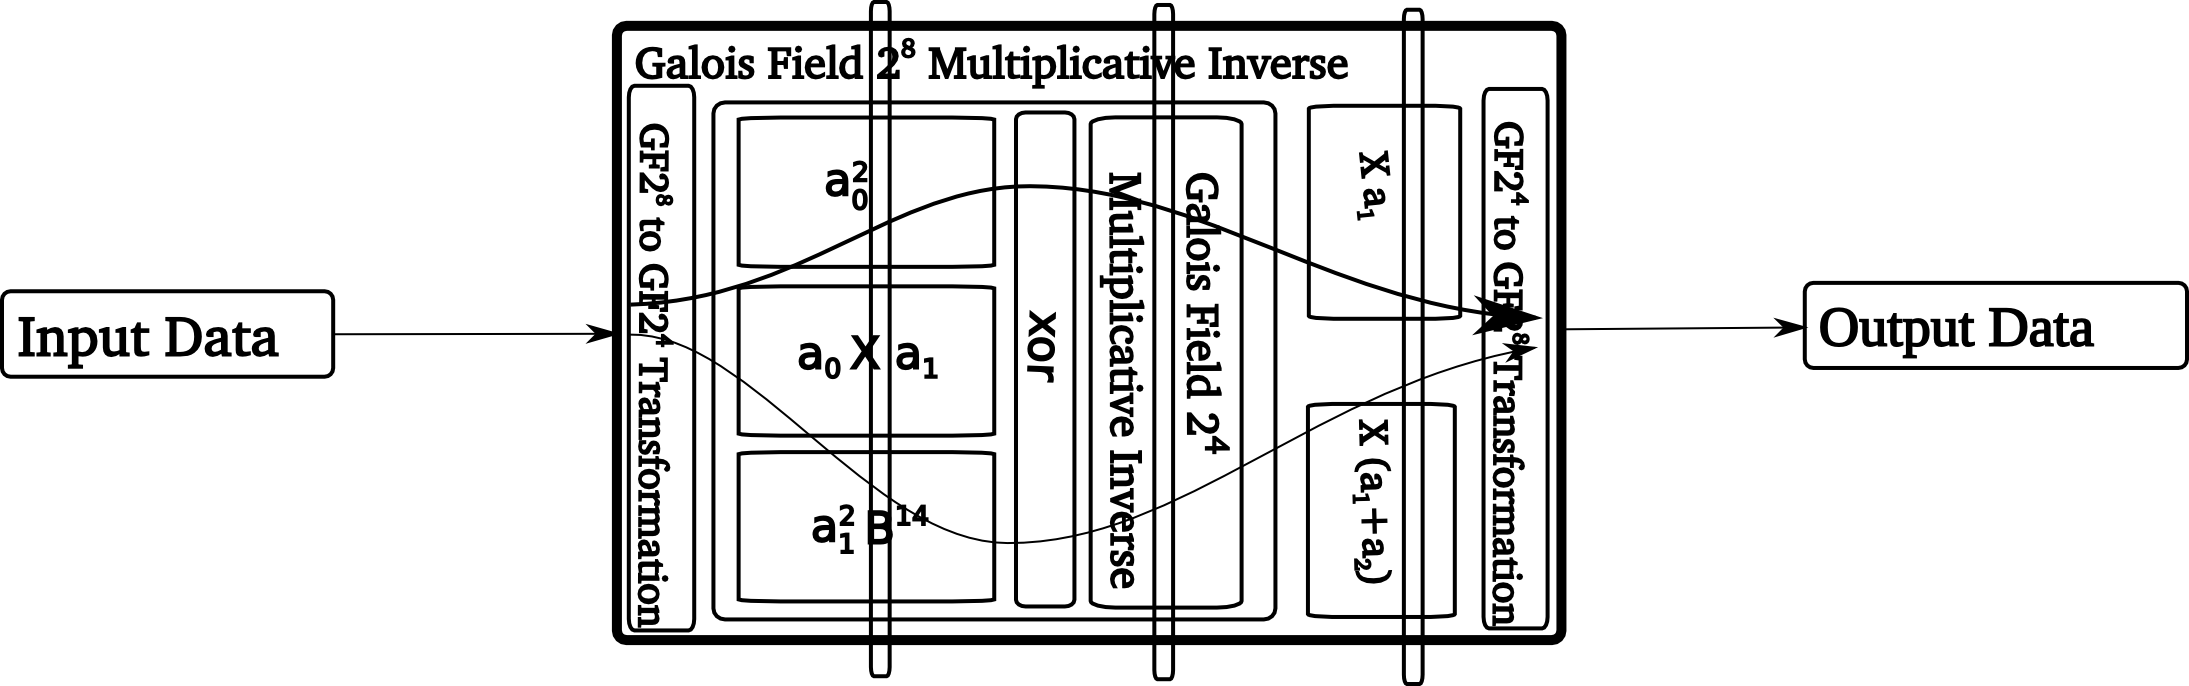
\includegraphics[width=0.75 \textwidth]{composite.png}
\caption{GF $2^8$ inversion by using composite field}
\label{composite}
\end{figure}

\begin{figure}
\centering
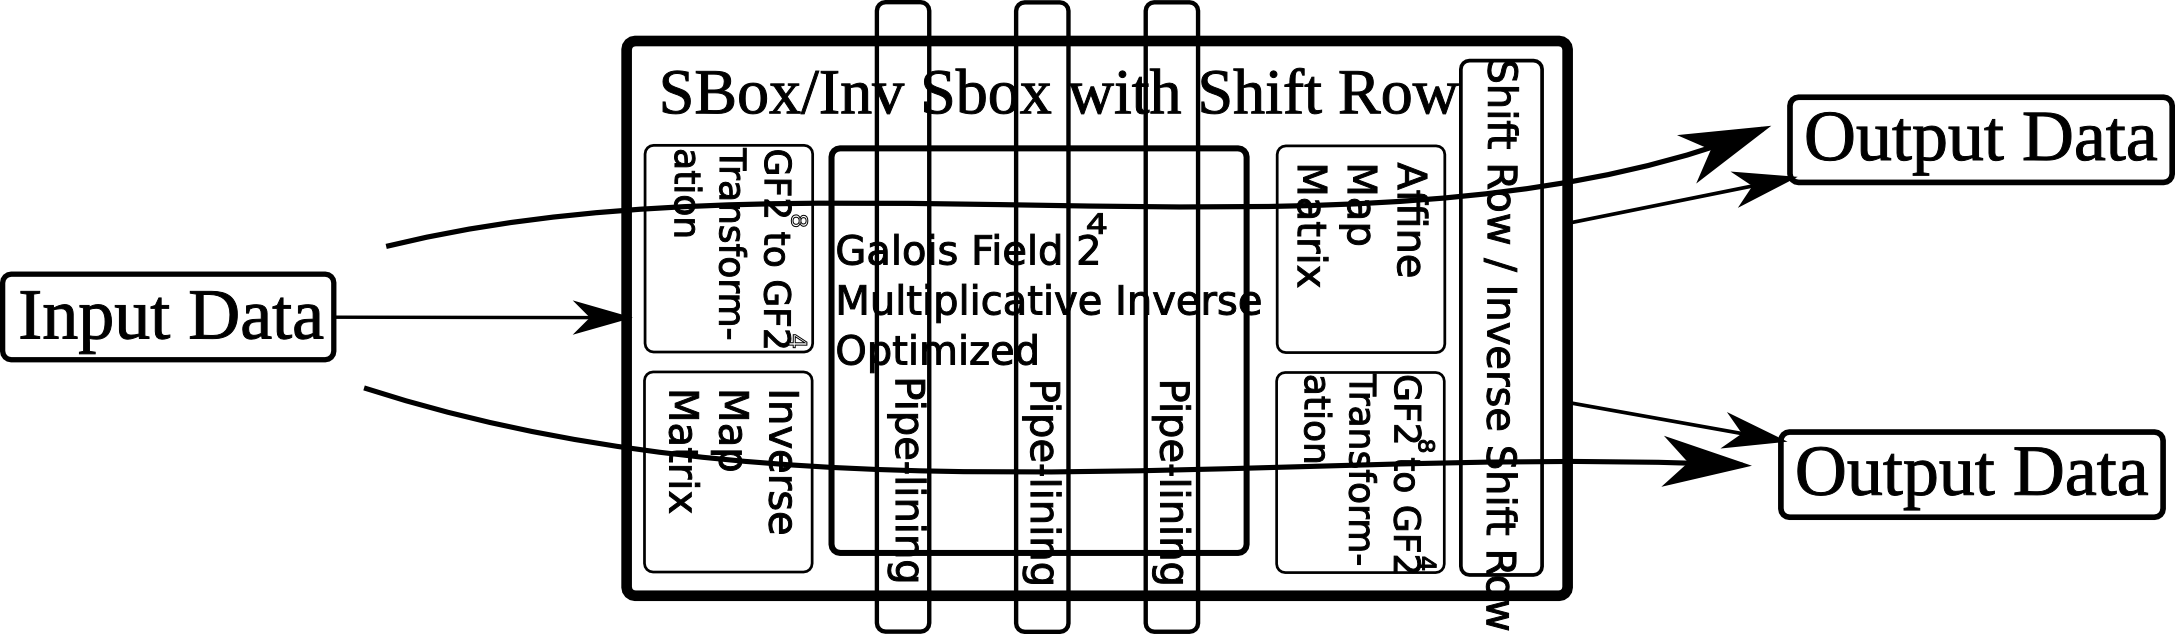
\includegraphics[width=0.75 \textwidth]{sbox.png}
\caption{Sbox module merged with shift module}
\label{Sbox}
\end{figure}

\section{ShiftRows Transformation}
\label{sec:shift}

In the ShiftRow transformation, the bytes in the last three rows of the State are cyclically shifted over different numbers of bytes (offsets). The first row, r = 0, is not shifted. Specifically, the ShiftRow transformation proceeds as follows:

\begin{equation}
s_{r,c}'~ = ~s_{r,(c+shift(r,Nb))mod Nb}  ~ for ~0<r<4~ and ~0\leq c <Nb~
\label{eq:sub3}
\end{equation}
where the shift value shift(r,Nb) depends on the row number, r, as follows (recall that Nb = 4): 
\begin{equation}
shift (1,4) = 1 ; shift (2,4) = 2 ; shift (3,4) = 3 
\label{eq:sub4}
\end{equation}
This has the effect of moving bytes to \textquotedblleft lower\textquotedblright  positions in the row (i.e., lower values of c in a given row), while the \textquotedblleft lowest\textquotedblright  bytes wrap around into the \textquotedblleft top\textquotedblright  of the row (i.e., higher values of c in a given row). 
Shift Row have been implemented with the help of bus multiplexers.

This process operates individually on rows with individual offset byte.  The transform throughput is 32 bits per clock cycle and can be pipelined for column order. For a wider data path (128-bit) or the higher throughput such as 128 bits per clock cycle, multiplexers are not necessary. In 128-bit design Shift Row is merged in the Substitution module. Refer to the (figure:\ref{Sbox}). Thus simplifying the design and eliminating some multiplexers and reducing the size.

\section{MixColumn Transformation\cite{1512188}}
\label{sec:mix}

The MixColumn transformation operates on the State column-by-column, treating each column as a four-term polynomial. The columns are considered as polynomials over $GF(2^8)$ and multiplied modulo $x^4 + 1$ with a fixed polynomial a(x), given by 
\begin{equation}
a(x) = \{03\}~x^3 ~+ ~\{01\}~x^2 ~+ ~\{01\}~x ~+ ~\{02\}
\label{eq:sub5}
\end{equation}

This can be written as a matrix multiplication. Let 

$s'(x) = a (x) \oplus s(x)~ :$ 
\begin{equation}
\left[ \begin{array}{c}
s_{0,c}' \\s_{1,c}' \\s_{2,c}' \\s_{3,c}' \end{array} \right] =
\left[ \begin{array}{cccccccc}
02 & 03 & 01 & 01\\
01 & 02 & 03 & 01\\
01 & 01 & 02 & 03\\
03 & 01 & 01 & 02\\
 \end{array} \right] \oplus
 \left[ \begin{array}{c}
s_{0,c}\\s_{1,c}\\s_{2,c}\\s_{3,c} \end{array} \right]
\label{eq:sub6}
\end{equation}

\subsection {InvMixColumn Transformation}
\label{sec:invmix}

InvMixColumn is the inverse of the MixColumns transformation. InvMixColumn operates on the State column-by-column, treating each column as a four-term polynomial. The columns are considered as polynomials over $GF(2^8)$ and multiplied modulo $x^4 + 1 $ with a fixed polynomial $a^-1(x)$, given by 
\begin{equation}
a^{-1}(x) = \{0b\}x^3 + \{0d\}x^2 + \{09\}x + \{0e\}
\end{equation}
this can be written as a matrix multiplication. Let 
$s'(x) = a^{−1}(x) \oplus s(x)~ :$
\begin{equation}
\left[ \begin{array}{c}
s_{0,c}' \\s_{1,c}' \\s_{2,c}' \\s_{3,c}' \end{array} \right] =
\left[ \begin{array}{cccccccc}
0e & 0b & 0d & 09\\
09 & 0e & 0b & 0d\\
0d & 09 & 0e & 0b\\
0b & 0d & 09 & 0e\\
 \end{array} \right] \oplus
 \left[ \begin{array}{c}
s_{0,c}\\s_{1,c}\\s_{2,c}\\s_{3,c} \end{array} \right]
\end{equation}

we can see that coefficients of $a^{-1}$ are more complex than coefficients of $a(X)$.As a result, hardware implementing AES decryption is larger and slower than for encryption. In order to reduce hardware cost, the InvMixColumn can be decomposed to share logic resources with MixColumn.

\subsection {Byte-Level Resource Sharing in MixColumn}
The first byte of the MixColumn implementation based on byte-level resource sharing  

\begin{equation}
b_0~=~\{02\}~a_0~+~\{03\}~a_1~+~a_2~+~a_3~
\end{equation}

Multiplication in algebraic fields is distributive over addition. This property enables byte-level resource sharing. I can further reduce this equation to
\begin{equation}
\Rightarrow ~(~a_0~+~a_1~+~a_2~+~a_3~)~+~\{02\}~(~a_0~+~a_1~)~+~a_0
\end{equation}
the term a0+ a1 + a2 + a3 can be shared by all four bytes of the MixColumn function.
\begin{eqnarray}
b0~=~(~a_0~+~a_1~+~a_2~+~a_3~)~+~\{02\}~(~a_0~+~a_1~)~+~a_0\\
b1~=~(~a_0~+~a_1~+~a_2~+~a_3~)~+~\{02\}~(~a_1~+~a_2~)~+~a_1\\
b2~=~(~a_0~+~a_1~+~a_2~+~a_3~)~+~\{02\}~(~a_2~+~a_3~)~+~a_2\\
b3~=~(~a_0~+~a_1~+~a_2~+~a_3~)~+~\{02\}~(~a_3~+~a_0~)~+~a_3\\
\end{eqnarray}
\subsection {Byte-Level Resource Sharing in InvMixColumn}
The first byte of inverse mix column is

$b_0'~=~\{0E\}~a_0~+~\{0B\}~a_1~+~\{0D\}~a_2~+~\{09\}~a_3$
\begin{figure}
  \centering
    \includegraphics[width=0.50\textwidth]{mtech/gifs/mix2.png}
  \caption{Multi Level Resource Sharing}
  \label{mix2}
\end{figure}
it can be further expanded as

\begin{equation}
b_0'{}=\{02\}(a_0+a_1)+a_1+a_2+a_3+\{04\}(\{02\}(a_0+a_1)+\{02\}(a_2+a_3)+(a_0+a_2))
\end{equation}

where 
\begin{align}
(\{02\}(a_0+a_1)+\{02\}(a_2+a_3)+(a_0+a_2))\\
\Rightarrow \{03\}a_0+\{02\}a_1+\{03\}a_2+\{03\}a_3\\
\Rightarrow(\{02\}a_0+\{03\}a_1+a_2+a_3)~+~(a_0+a_1+\{03\}a_2+\{02\}a_3)\\
\Rightarrow b_0+b_2
\end{align}
and
\begin{align}
\{02\}(a_0+a_1)+a_1+a_2+a_3\\
\Rightarrow \{02\}(a_0+a_1)+a_1+a_2+a_3+bold{a_0}~bold{+a_0}\\
\Rightarrow b_0
\end{align}
so
\begin{equation}
b_0'=b_0+\{04\}(b0+b2)
\end{equation}
similarly\\
\begin{align}
b_1'=b_1+\{04\}(b1+b3)\\
b_2'=b_2+\{04\}(b0+b2)\\
b_3'=b_3+\{04\}(b1+b3)
\end{align}

in this way it can be shown that Inv Mix Column is related to Mix column and further logic can be reduced order of times by resource sharing. 

In the (figure:\ref {mix2}) the scheme is shown for Multilevel Resource Sharing for Mixcolumn and inverse mixcolumn.

\section{Core Design}
Initially 32 bit core is designed. In this design each transformation takes 4 cycles. State buffer is designed in a special way so that it can work in three modes. (1) Column mode, (2) Row mode and (3) memory block mode. In memory block mode data is transferred in blocks to/from State from/to the main memory buffer.

Design has one accumulator named out\_ register. Transformation can be performed in either way (1)  State - core transformation - out\_ register, (2) out\_ register - core transformation - State, By the help of this shuttle mechanism lot of time is being saved from saving the result again in the State. 

All the transformations (sub byte, Mix column .etc) are implemented in aes\_ modules as a memory device. That means different address of aes\_ modules corresponds to different transformation.

\subsection{128 bit Core Design}
Further for higher throughput a new design with 128 bit wide data bus is designed. In this each transformation is done in a state array in a single cycle. Thus increased throughput and reduced complexity. 
%%%%%%%%%%%%%%%%%%%%%%%%%%%%%%%%%%%%%%%%%%%%%%%%
%% SECTION
%%%%%%%%%%%%%%%%%%%%%%%%%%%%%%%%%%%%%%%%%%%%%%%%
\section{Performance and Comparisons}
Various Design\cite{SumioMorioka} of S-boxes are studied along with S-boxes which are developed in this project in (table:\ref{tab:b}) (figure:\ref{Throusizcmp1}) and their size verses delay comparisons are done. In (figure:\ref{Throusizcmp1}) Green and Red dot represents designs developed during this projects and are based on Galois field inversion. Blue dots represent designs from a paper \cite{SumioMorioka} where Satoh discussed different designs methodology. These design are basically ASIC Designs that's why delays are very less in contrast with the designs in this project as they are FPGA based. Implementing these designs in ASIC may further reduce the delays. Red dots represents the most optimum design with respect to size and delay.

\begin{table}
\begin{tabular}{lrrrr}
\hline
  \tablehead{1}{l}{b}{Sbox}
  & \tablehead{1}{r}{b}{Total CLB}
  & \tablehead{1}{r}{b}{1/delay Mhtz}
  & \tablehead{1}{r}{b}{Throughput \\per unit Size\\ = Freq/CLB}   \\
\hline
Euclidean & 140 & 99.80 & 0.71\\
Euclidean\_1\_Pipeline & 149 & 88.50 & 0.59\\
Euclidean\_2\_Pipeline & 178 & 64.85 & 0.36\\
Euclidean\_4\_Pipeline & 211 & 215.05 & 1.02\\
Sbox+Inv\_EUC\_4\_pline & 110 & 215.05 & 1.96\\
Composite\_GF & 48 & 71.94 & 1.50\\
Composite\_GF\_2\_Pline & 79 & 150.83 & 1.91\\
Composite\_GF\_4\_Pline & 81 & 277.01 & 3.42\\
Sbox+Inv\_CGF\_4\_pline & 47.5 & 277.01 & 5.83\\
PPRM & 2148 & 990.09 & 0.46\\
SOP & 1567 & 1298.70 & 0.83\\
LUT & 1528 & 1428.57 & 0.93\\
BDD & 1399 & 1449.28 & 1.04\\
TBDD & 2818 & 2325.58 & 0.83\\
\hline
\end{tabular}
\caption{Size, Max Frequency and Throughput per Unit Size comparision of different implementations}
\label{tab:b}
\end{table}

further size delay comparison is done between different designs of S-boxes which are developed in this project in (table:\ref{tab:b}) (figure:\ref{Throusizcmp1})

\begin{figure}
\centering
{\includegraphics[ scale=0.5]{mtech/gifs/Throusizcmp3.png}}%
\caption{Delay Vs CLB Comparison Between Different Architectures}
\label{Throusizcmp1}
\end{figure}

\begin{table}
\begin{tabular}{lrrrr}
\hline
  \tablehead{1}{r}{b}{}
  & \tablehead{1}{r}{b}{Devices}
  & \tablehead{1}{r}{b}{CLB Slices}
  & \tablehead{1}{r}{b}{Throughput(Mbits/Sec)}   \\
\hline
Ichikawa \cite{ICHIKAWA}& VLSI & & 1950\\
Weeks \cite{Week}& VLSI & & 1950\\
Lutz \cite{LUTZ} & VLSI & & 2263\\
Elbirt& xcv1000 \cite{ELBIRT}& 9004 & 1940\\
McLoone and McCanny& XCV3200E \cite{MCLOONE}& 7576 & 3239\\
E Rodriguez-Henriquez\cite{citeulike341092}& XCV2000E & 5677+80 Brams & 4129\\
This Design& XC4VFX12 & 3206 & 3315.2\\
\hline
\end{tabular}
\caption{Size and Delay comprison of different Core Implementations studied with
this design}
\label{tab:a}
\end{table}

\subsection{Comparison with Micro-controllers}
Micro-controllers\index{micro-controllers} and micro processors are general purpose devices generally used for general purpose computing. They are made to be a universal state-machines. Generally they have ALU , Multipliers Internal registers and memory catches hence lot of equivalent gates. A typical P4 Processor contains 55 Million gates. In contrast with FPGA Design those are generally application specific using much fewer resources.

As controllers are ASIC they works on Gigahertz Clocks whereas a typical FPGA works on 100 Mhz Clock. So in order to compare between the two we have to device a different bench mark.

Comparison done is based on number of clocks a core takes to encrypt a single byte (see (Table:\ref{tab:c})). Throughput are taken for different available architectures with a standard Openssl Speed Aes tool\cite{Bernsteinnewaes}.

\begin{table}
\begin{tabular}{lrrrr}
\hline
  \tablehead{1}{l}{b}{Core}
  & \tablehead{1}{r}{b}{Clocks/Byte}
  & \tablehead{1}{r}{b}{Throughput \\ Mbit/sec}\\
\hline
Motorola PowerPC G4 7410, \\ ppc32 architecture  & 29 & 147.03 \\
Intel Pentium 4 f12, x86 \\architecture & 21 & 723.81 \\
Sun UltraSPARC III, sparcv9 \\architecture  & 35 & 205.71 \\
Intel Core 2 Quad Q6600 6fb, \\amd64 architecture& 18 & 1066.67 \\
AMD Athlon 64 X2 3800+ \\15/75/2, amd64 architecture & 21 & 761.9 \\
This Design with 128bit bus size & 0.63 & 3315.2 \\
This Design with 32bit bus size & 2.5 & 828.8 \\
\hline
\end{tabular}
\caption{Comparison of Cycles / unit byte encryption between different
Processors Architectures}
\label{tab:c}
\end{table}

\paragraph{Throughput Calculation for 128 bit Bus Size }
\begin{eqnarray*}\label{xx}
Max. Delay & = 3.86 nano Sec. & = 3.86 \times 10^{-9} Sec \\
Max.Frequency & = \frac{1}{ 3.86 \times 10^{-9}} Hz \\
&= 259 \times 10^6 Hz \\
Throughput &= \frac{[Bus Width] \times [Frequency]} {[No Of Rounds]} \\
&= 3315.2 \times 10^6 bits/sec
\end{eqnarray*}

%%%%%%%%%%%%%%%%%%%%%%%%%%%%%%%%%%%%%%%%%%%%%%%%
%% SECTION&= \frac{128 \times 259 \times 10^6} {10} \\
%%%%%%%%%%%%%%%%%%%%%%%%%%%%%%%%%%%%%%%%%%%%%%%%

\section{Conclusion}

\begin{figure}
  \includegraphics[ scale=0.25]{mtech/gifs/multichannel.png}%
  \caption{Different Modes}
\end{figure}


During the development of this project number of different FPGA based architectures are studied. This study is done on the basis of Design size and throughput. Among them, architecture based on composite field arithmetic is selected due to very compact design with moderate delays. 

Hard-wire ShiftRow (and Inverse ShiftRow) operation in the sbox and byte level resource sharing between mix column and inverse mix column lead to both good speed and area saving.

All the transformations are optimized in the time domain by introducing pipelining in the transforms having larger gate depth.

Further Multiple parallel transform blocks are used in 32 bit and 128 bit designs in order to achieve parallelism. Alternatively, processing speed could be made higher by employing gate array or standard cell technology.

However, one should note that the pipeline structure is suitable for ECB (Electronic Code Book) mode of operation, but not very useful for other three modes (BCB, CFB, and OFB mode) where feedbacks are employed.
 
But in this design these feedback mode problem is taken care by dividing the pipelined channel into different independent parallel channels. Now these channels can work in (BCB, CFB, and OFB mode) feedback mods independently with lower throughputs. But total combined throughput of the design in these feedback modes will be equivalent to the throughput of design working as single channel in ECB mode.

This technique is quite suitable for servers who have to make different multiple encrypted sessions with multiple clients. Their high network throughput is required due to multiple clients. But in a single session high throughput is not required.


%%%%%%%%%%%%%%%%%%%%%%%%%%%%%%%%%%%%%%%%%%%%%%%%
%% BACKMATTER
%%%%%%%%%%%%%%%%%%%%%%%%%%%%%%%%%%%%%%%%%%%%%%%%

%\begin{theacknowledgments}
%  Infandum, regina, iubes renovare dolorem, Troianas ut opes et
%  lamentabile regnum cruerint Danai; quaeque ipse miserrima vidi, et
%  quorum pars magna fui. Quis talia fando Myrmidonum Dolopumve aut duri
%  miles Ulixi temperet a lacrimis?
%\end{theacknowledgments}

%%%%%%%%%%%%%%%%%%%%%%%%%%%%%%%%%%%%%%%%%%%%%%%%
%% The bibliography can be prepared using the BibTeX program or
%% manually.
%%
%% The code below assumes that BibTeX is used.  If the bibliography is
%% produced without BibTeX comment out the following lines and see the
%% aipguide.pdf for further information.
%%
%% For your convenience a manually coded example is appended
%% after the \end{document}
%%%%%%%%%%%%%%%%%%%%%%%%%%%%%%%%%%%%%%%%%%%%%%%%

%%%%%%%%%%%%%%%%%%%%%%%%%%%%%%%%%%%%%%%%%%%%%%%%
%% You may have to change the BibTeX style below, depending on your
%% setup or preferences.
%%
%%
%% For The AIP proceedings layouts use either
%%%%%%%%%%%%%%%%%%%%%%%%%%%%%%%%%%%%%%%%%%%%

\bibliographystyle{aipproc}   % if natbib is available
%\bibliographystyle{aipprocl} % if natbib is missing

%%%%%%%%%%%%%%%%%%%%%%%%%%%%%%%%%%%%%%%%%%%
%% You probably want to use your own bibtex database here
%%%%%%%%%%%%%%%%%%%%%%%%%%%%%%%%%%%%%%%%%%%
\bibliography{thesis}

%%%%%%%%%%%%%%%%%%%%%%%%%%%%%%%%%%%%%%%%%%%
%% Just a reminder that you may have to run bibtex
%% All of it up to \end{document} can be removed
%% if you don't like the warning.
%%%%%%%%%%%%%%%%%%%%%%%%%%%%%%%%%%%%%%%%%%%
\IfFileExists{\jobname.bbl}{}
 {\typeout{}
  \typeout{******************************************}
  \typeout{** Please run "bibtex \jobname" to optain}
  \typeout{** the bibliography and then re-run LaTeX}
  \typeout{** twice to fix the references!}
  \typeout{******************************************}
  \typeout{}
 }

\end{document}


\endinput
%%
%% End of file `template-8s.tex'.
